\documentclass{beamer}
%\usepackage{xspace}
\usepackage{amsmath,amssymb}
\usepackage{graphicx}
%\usepackage{svg}
%\usepackage{pgfpages}
%\pgfpagesuselayout{4 on 1}[a4paper,border shrink=5mm,landscape]
%\usepackage{psfrag}
%\usepackage[usenames,dvipsnames]{xcolor}
\usepackage{braket}
\usepackage{qcircuit}
\usepackage{tikz}
\usetikzlibrary{circuits.logic.US}
\usetikzlibrary{graphs}
\usetikzlibrary{datavisualization}
\usetikzlibrary{datavisualization.formats.functions}
\usepackage{pgfplotstable}
\usepgfplotslibrary{patchplots}

\setbeamercovered{transparent}

\usetheme{Pittsburgh}
%\usetheme{default}

\setbeamertemplate{sidebar right}{}
\setbeamertemplate{footline}[frame number]
%\usefonttheme{professionalfonts}

%\usepackage{sansmathaccent}
%\usepackage{bm}

%\usepackage{unicode-math}
%%\setmainfont[SlantedFont={Latin Modern Roman Slanted},SlantedFeatures={Color=000000},
%%  SmallCapsFont={TeX Gyre Termes},SmallCapsFeatures={Letters=SmallCaps}]{XITS}
%\setmathfont[math-style=ISO,sans-style=upright]{XITS Math}
%\setmathfont[range={\mathcal,\mathbfcal}]{Latin Modern Math}

\usepackage{sfmath}

%\mathversion{sans}

\newcommand{\Tr}{\mathsf{Tr}}

\definecolor{redorange}{rgb}{1.0, .25, .25}
\definecolor{citation}{rgb}{.1, 0.8, .35}
\newcommand\emm[1]{\textcolor{redorange}{{#1}}}
\newcommand\numc[1]{\textcolor{citation}{{\bf #1}}}

%\newcommand\bm[1]{{\mbox{\boldmath $#1$}}}
\newcommand\bm[1]{{\mathbf{#1}}}
%\newcommand\bm[1]{{\bf #1}}
%\newcommand\bm[1]{\ensuremath{\boldsymbol{#1}}}
%\newcommand\bm[1]{{\textbf{\it #1}}}

\title{Universality of quantum circuit}
\author{Ryuhei Mori}
%\institute{$\vcenter{\hbox{\includegraphics[width=30pt]{ELC_logo}}}$ Postdoctoral Fellow of ELC\\ $\vcenter{\hbox{\includegraphics[width=20pt]{titech_logo}}}$ Tokyo Institute of Technology}
\institute{Tokyo Institute of Technology}
%\date{21, Feb, 2019}



\begin{document}
\begin{frame}[plain]
\maketitle
\end{frame}



\begin{frame}{Boolean circuit}
\begin{itemize}
\setlength{\itemsep}{2em}
\item Boolean function $f\colon \{0,1\}^n\to\{0,1\}$.
\item \emm{Boolean circuit} is a model of computation of a Boolean functions which consists of logic \emm{gates}.
\item AND gate:
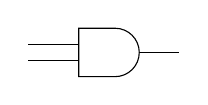
\begin{tikzpicture}[circuit logic US, baseline]
\node[and gate] (A) {};
\foreach \a in {1, 2}
  \draw (A.input \a -| -1,0) -- (A.input \a);
\draw (A.output) -- ([xshift=0.5cm]A.output);
\end{tikzpicture}
\item OR gate:
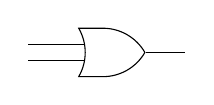
\begin{tikzpicture}[circuit logic US, baseline]
\node[or gate] (A) {};
\foreach \a in {1, 2}
  \draw (A.input \a -| -1,0) -- (A.input \a);
\draw (A.output) -- ([xshift=0.5cm]A.output);
\end{tikzpicture}
\item NOT gate:
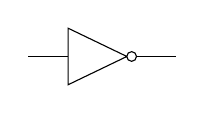
\begin{tikzpicture}[circuit logic US, baseline]
\node[not gate] (A) {};
\draw (A.input) -- ([xshift=-0.5cm]A.input);
\draw (A.output) -- ([xshift=0.5cm]A.output);
\end{tikzpicture}
\end{itemize}
\end{frame}

\begin{frame}{Universality of a quantum circuit}
\begin{theorem}[Universality of finite gate set]
For any unitary matrix $U\in L(\mathbb{C}^{2^n})$ and $\emm{\epsilon} >0$,
there is a quantum circuit with \emm{$X,\,Y,\,Z,\,H,\,S,\,\mathsf{CNOT},\,\mathsf{Toffoli}$} gates computing $\widetilde{U}$
satisfying $\|U-\widetilde{U}\|<\emm{\epsilon}$.
\end{theorem}
\begin{proof}
\begin{enumerate}
\setlength{\itemsep}{1em}
\item Any unitary matrix can be decomposed to a product of \emm{two-level unitary matrices}.
\item Any two-level unitary matrix can be decomposed to a product of \emm{CNOT and controlled-unitary gates}.
\item Any controlled-untary gate can be decomposed to a product of \emm{CNOT and arbitrary single-qubit gates}.
\item Any single-qubit gate can be approximated by $X,\,Y,\,Z,\,H,\,S$ and $T$.
\end{enumerate}
\end{proof}
\end{frame}

\begin{frame}{Two-level unitary matrix}
\begin{equation*}
\begin{bmatrix}
1&0&0&0&0&0&0&0&0\\
0&1&0&0&0&0&0&0&0\\
0&0&\emm{u_{11}}&0&0&0&0&\emm{u_{12}}&0\\
0&0&0&1&0&0&0&0&0\\
0&0&0&0&1&0&0&0&0\\
0&0&0&0&0&1&0&0&0\\
0&0&0&0&0&0&1&0&0\\
0&0&\emm{u_{21}}&0&0&0&0&\emm{u_{22}}&0\\
0&0&0&0&0&0&0&0&1\\
\end{bmatrix}
\end{equation*}
\end{frame}

\begin{frame}{Two-level unitary matrix}
\begin{theorem}[Decomposition to two-level unitary matrices]
For any unitary matrix $U\in L(\mathbb{C}^{d})$, there is a sequence $U_1,\,U_2,\,\dotsc,\,U_m$ of \emm{two-level unitary matrices} such that
$U=U_1U_2\dotsm U_m$.
\end{theorem}
\begin{proof}
We will show that there is a sequence $V_1,\,V_2,\,\dotsc,\,V_m$ of two-level unitary matrices such that
\begin{equation*}
V_m V_{m-1}\dotsm V_1 U = I.
\end{equation*}
Since $U_i := V_i^{-1}$ is two-level unitary, this completes a proof.
\end{proof}
\end{frame}

\begin{frame}{Decomposition to two-level unitary matrix 1/3}
\begin{equation*}
U=
\begin{bmatrix}
\emm{u_{1,1}}&u_{1,2}&u_{1,3}&u_{1,4}\\
u_{2,1}&u_{2,2}&u_{2,3}&u_{2,4}\\
u_{3,1}&u_{3,2}&u_{3,3}&u_{3,4}\\
u_{4,1}&u_{4,2}&u_{4,3}&u_{4,4}
\end{bmatrix}
\end{equation*}
If $u_{1,1}\ne 0$, we skip the first step.

If $u_{1,1}= 0$, there exists $i\in\{2,3,\dotsc,d\}$ such that $u_{d,1}\ne 0$.
Apply the two-level permutation matrix
\begin{equation*}
V=
\begin{bmatrix}
0&0&0&\emm{1}\\
0&1&0&0\\
0&0&1&0\\
\emm{1}&0&0&0
\end{bmatrix}
\end{equation*}
which swap the first row and the $d$-th row.
\end{frame}

\begin{frame}{Decomposition to two-level unitary matrix 2/3}
\begin{equation*}
U=
\begin{bmatrix}
u_{1,1}&u_{1,2}&u_{1,3}&u_{1,4}\\
\emm{u_{2,1}}&u_{2,2}&u_{2,3}&u_{2,4}\\
u_{3,1}&u_{3,2}&u_{3,3}&u_{3,4}\\
u_{4,1}&u_{4,2}&u_{4,3}&u_{4,4}
\end{bmatrix}
\end{equation*}
If $u_{2,1}= 0$, we skip this step.

If $u_{2,1}\ne 0$, apply the two-level unitary matrix
\begin{equation*}
V=
\frac1{|u_{1,1}|^2+|u_{2,1}|^2}
\begin{bmatrix}
u_{1,1}^*&u_{2,1}^*&0&0\\
\emm{-u_{2,1}}&\emm{u_{1,1}}&0&0\\
0&0&|u_{1,1}|^2+|u_{2,1}|^2&0\\
0&0&0&|u_{1,1}|^2+|u_{2,1}|^2
\end{bmatrix}
\end{equation*}
\end{frame}

\begin{frame}{Decomposition to two-level unitary matrix 2'/3}
\begin{equation*}
U=
\begin{bmatrix}
u_{1,1}&u_{1,2}&u_{1,3}&u_{1,4}\\
0&u_{2,2}&u_{2,3}&u_{2,4}\\
\emm{u_{3,1}}&u_{3,2}&u_{3,3}&u_{3,4}\\
u_{4,1}&u_{4,2}&u_{4,3}&u_{4,4}
\end{bmatrix}
\end{equation*}
If $u_{2,1}= 0$, we skip this step.

If $u_{2,1}\ne 0$, apply the two-level unitary matrix
\begin{equation*}
V=
\frac1{|u_{1,1}|^2+|u_{3,1}|^2}
\begin{bmatrix}
u_{1,1}^*&0&u_{3,1}^*&0\\
0&|u_{1,1}|^2+|u_{3,1}|^2&0&0\\
\emm{-u_{3,1}}&0&\emm{u_{1,1}}&0\\
0&0&0&|u_{1,1}|^2+|u_{3,1}|^2
\end{bmatrix}
\end{equation*}
\end{frame}

\begin{frame}{Decomposition to two-level unitary matrix 3/3}
\begin{equation*}
U=
\begin{bmatrix}
u_{1,1}&u_{1,2}&u_{1,3}&u_{1,4}\\
0&u_{2,2}&u_{2,3}&u_{2,4}\\
0&u_{3,2}&u_{3,3}&u_{3,4}\\
0&u_{4,2}&u_{4,3}&u_{4,4}
\end{bmatrix}
=
\begin{bmatrix}
u_{1,1}&0&0&0\\
0&\emm{u_{2,2}}&u_{2,3}&u_{2,4}\\
0&u_{3,2}&u_{3,3}&u_{3,4}\\
0&u_{4,2}&u_{4,3}&u_{4,4}
\end{bmatrix}
\end{equation*}

\vspace{2em}
\centering
\large
Arbitrary $d\times d$ unitary matrix can be decomposed to product of at most $(d+1)d/2$ two-level unitary matrices.
\end{frame}

\begin{frame}{Universality of a quantum circuit}
\begin{theorem}[Universality of finite gate set]
For any unitary matrix $U\in L(\mathbb{C}^{2^n})$ and $\emm{\epsilon} >0$,
there is a quantum circuit with \emm{$X,\,Y,\,Z,\,H,\,S,\,\mathsf{CNOT},\,\mathsf{Toffoli}$} gates computing $\widetilde{U}$
satisfying $\|U-\widetilde{U}\|<\emm{\epsilon}$.
\end{theorem}
\begin{proof}
\begin{enumerate}
\setlength{\itemsep}{1em}
\item Any unitary matrix can be decomposed to a product of \emm{two-level unitary matrices}. {\color{green}{Done}}
\item Any two-level unitary matrix can be decomposed to a product of \emm{CNOT and controlled-unitary gates}.
\item Any controlled-untary gate can be decomposed to a product of \emm{CNOT and arbitrary single-qubit gates}.
\item Any single-qubit gate can be approximated by $X,\,Y,\,Z,\,H,\,S$ and $T$.
\end{enumerate}
\end{proof}
\end{frame}

\begin{frame}{Universality of a quantum circuit}
\begin{lemma}
Any $2^n\times 2^n$ two-level unitary matrix can be decomposed to a product of \emm{CNOT and controlled-unitary gates}.
\end{lemma}
\begin{proof}
Assume that the two-level unitary matrix acts on a 2-dimentional subspace $\mathsf{span}(\{\ket{x}, \ket{y}\})$ for $x\ne y \in\{0,1\}^n$.

\vspace{1em}
Assume that for $i\in\{1,2,\dotsc,n\}$, $x_i = 1$ and $y_i = 0$.
\vspace{1em}
Apply at most $n-1$ CNOT gates such that
\begin{align*}
\ket{x}&\longmapsto \ket{\emm{y\oplus e_i}}\\
\ket{y}&\longmapsto \ket{y}
\end{align*}
Then, apply \emm{``controlled unitary''} and reverse the permutation of the basis.
\end{proof}
\end{frame}

\begin{frame}{Example of the first part}
Let $x = \mathtt{00\emm{1}01},\, y = \mathtt{11\emm{0}00}$.
\[
\Qcircuit @C=2em @R=2em {
\lstick{\ket{0}} & \targ & \qw &\qw & \rstick{\ket{1}}\qw \\
\lstick{\ket{0}} & \qw & \targ &\qw &\rstick{\ket{1}}\qw \\
\lstick{\ket{1}} & \ctrl{-2} & \ctrl{-1} &\ctrl{2} &\rstick{\ket{1}}\qw \\
\lstick{\ket{0}} & \qw & \qw &\qw &\rstick{\ket{0}}\qw \\
\lstick{\ket{1}} & \qw & \qw &\targ &\rstick{\ket{0}}\qw
}
\]
\begin{align*}
\ket{00101}&\longmapsto \ket{11\emm{1}00}\\
\ket{11000}&\longmapsto \ket{11\emm{0}00}
\end{align*}
\end{frame}

\begin{frame}{Controlled unitary}
\[
\Qcircuit @C=2em @R=2em {
& \ctrl{1} & \qw \\
& \gate{U} & \qw \\
}
\]

\[
\Qcircuit @C=2em @R=2em {
& \ctrlo{1} & \qw \\
& \gate{U} & \qw \\
}
\quad
= 
\quad
\Qcircuit @C=2em @R=2em {
& \gate{X} & \ctrl{1} & \gate{X} & \qw \\
& \qw & \gate{U} & \qw & \qw \\
}
\]

\vspace{1em}
\[
\Qcircuit @C=2em @R=2em {
& \ctrl{1} & \qw \\
& \ctrl{1} & \qw \\
& \ctrl{1} & \qw \\
& \gate{U} & \qw \\
}
\]
\end{frame}

\begin{frame}{Idea of the last part}
\vspace{-1.5em}
\begin{align*}
\ket{x}=\ket{00101}&\longmapsto \ket{11\emm{1}00}\\
\ket{y}=\ket{11000}&\longmapsto \ket{11\emm{0}00}
\end{align*}
\[
\Qcircuit @C=2em @R=2em {
\lstick{\ket{1}} & \ctrl{1} & \qw \\
\lstick{\ket{1}} & \ctrl{1} & \qw \\
\lstick{\ket{1}} & \gate{U} & \qw \\
\lstick{\ket{0}} & \ctrlo{-1} & \qw \\
\lstick{\ket{0}} & \ctrlo{-1} & \qw 
}
\]

\vspace{1em}
Finally, reverse the basis
\begin{align*}
\ket{11\emm{1}00}&\longmapsto \ket{00101}=\ket{x}\\
\ket{11\emm{0}00}&\longmapsto \ket{11000}=\ket{y}
\end{align*}
\end{frame}

\begin{frame}{Whole quantum circuit}
Let $x = \mathtt{00\emm{1}01},\, y = \mathtt{11\emm{0}00}$.
\[
\Qcircuit @C=2em @R=2em {
 & \targ & \qw &\qw & \ctrl{1} & \qw & \qw & \targ &\qw \\
 & \qw & \targ &\qw & \ctrl{1} &\qw & \targ & \qw &\qw \\
 & \ctrl{-2} & \ctrl{-1} &\ctrl{2} & \gate{U} &\ctrl{2} & \ctrl{-1} & \ctrl{-2} & \qw \\
 & \qw & \qw &\qw & \ctrlo{-1} &\qw & \qw & \qw & \qw \\
 & \qw & \qw &\targ & \ctrlo{-1} &\targ & \qw & \qw & \qw
}
\]
\begin{align*}
\ket{00101}&\longmapsto \ket{11\emm{1}00}\\
\ket{11000}&\longmapsto \ket{11\emm{0}00}
\end{align*}
\end{frame}

\begin{frame}{Universality of a quantum circuit}
\begin{theorem}[Universality of finite gate set]
For any unitary matrix $U\in L(\mathbb{C}^{2^n})$ and $\emm{\epsilon} >0$,
there is a quantum circuit with \emm{$X,\,Y,\,Z,\,H,\,S,\,\mathsf{CNOT},\,\mathsf{Toffoli}$} gates computing $\widetilde{U}$
satisfying $\|U-\widetilde{U}\|<\emm{\epsilon}$.
\end{theorem}
\begin{proof}
\begin{enumerate}
\setlength{\itemsep}{1em}
\item Any unitary matrix can be decomposed to a product of \emm{two-level unitary matrices}. {\color{green}{Done}}
\item Any two-level unitary matrix can be decomposed to a product of \emm{CNOT and controlled-unitary gates}. {\color{green}{Done}}
\item Any controlled-untary gate can be decomposed to a product of \emm{CNOT and arbitrary single-qubit gates}.
\item Any single-qubit gate can be approximated by $X,\,Y,\,Z,\,H,\,S$ and $T$.
\end{enumerate}
\end{proof}
\end{frame}


\end{document}
